%  LaTeX support: latex@mdpi.com
%=================================================================
\documentclass[entropy,article,submit,pdftex,moreauthors]{Definitions/mdpi}

%=================================================================
% MDPI internal commands
\firstpage{1}
\makeatletter
\setcounter{page}{\@firstpage}
\makeatother
\pubvolume{1}
\issuenum{1}
\articlenumber{0}
\pubyear{2026}
\copyrightyear{2026}
\datereceived{ }
\daterevised{ }
\dateaccepted{ }
\datepublished{ }

%=================================================================
\Title{Hierarchy Depth Observables Predict Combinatorial Entropy in Finite Causal Posets: A Three-Tier Correlational Study}

\Author{Gang Zhang $^{1}$*}

\address{%
$^{1}$ \quad Independent Researcher; unicome@gmail.com}

\corres{Correspondence: unicome@gmail.com}

%=================================================================
\abstract{Companion papers (Predictions A and B) established that Lorentzian-like posets become competitive phases in action-weighted causal poset ensembles. What structural feature drives this advantage remains unexplained. We define a Hierarchy Integration Index (HII) --- a pre-registered composite z-score of five structural observables --- and test whether hierarchy depth predicts combinatorial entropy $\log H$ across three independent tiers: (i)~all-family exact computation (8 families, $N = 10$--$16$, 320 samples), (ii)~matched-pair $\Delta$-analysis (Lor2D vs MLR, 46 pairs, $N = 30$--$56$), and (iii)~coarse-graining identity-stability linkage (92 samples). At fixed $N$, deeper hierarchy correlates with lower $\log H$: partial $r = -0.578$ controlling for $N$; matched-pair $r = -0.834$, stable across three filter stringencies (variation $< 0.005$). Component decomposition reveals that \texttt{layer\_count} and \texttt{mean\_layer\_gap} carry most of the signal; the five-component HII composite never exceeds its best constituent. The mechanism chain extends to coarse-graining identity stability under the current classifier, with \texttt{layer\_count} predicting switch rate at $r = -0.874$. A Simpson's Paradox in the raw data ($r = +0.336$ before $N$ control) is diagnosed: $N$ is the dominant sign-determining confound. Hard limitations include family-specific HII reversals (KR-like, absolute-layered), classifier-dependent Tier~3, and weak near-wall power at $N \geq 52$. These results provide correlational support --- not causal demonstration --- for a link between hierarchy depth and entropy suppression in finite causal posets.}

\keyword{causal posets; hierarchy integration; combinatorial entropy; linear extensions; coarse-graining stability; Simpson's Paradox; causal set theory}

%=================================================================
\begin{document}

\section{Introduction}

\subsection{The ``Why Does Lor2D Win?'' Question}

Two companion papers have established the following finite-size results for discrete causal orders:

\begin{itemize}[nosep]
    \item \textbf{Prediction B}~\cite{zhang2026predB}: Using the same eight-family ensemble and action functional $\mathcal{A} = -\beta H + \gamma I$, the companion study shows that a two-dimensional Lorentzian-like (Lor2D) family becomes competitive against KR-like high-entropy posets at critical coupling $\gamma_c$ remaining $O(1)$ over $N = 10$--$44$. Non-target-anchored observable replacements preserve the competitive window. The key fact needed here: \emph{Lor2D achieves systematically lower $\log H$ than MLR at matched $N$, and this ordering is reproducible under action-score replacement.}

    \item \textbf{Prediction A}~\cite{zhang2026predA}: Replacing the target-anchored dimension penalty with a consistency constraint yields four-dimensional Lorentzian dominance in the majority of tested configurations, with a margin that grows with $N$ up to $N = 72$. The key fact needed here: \emph{dimensional selection and entropy ordering are connected, but the structural mechanism is unspecified --- which is the gap the present paper addresses.}
\end{itemize}

These results establish \emph{that} Lorentzian-like structures can dominate, and \emph{which} action terms drive the competition. They do not explain \emph{why} --- at the level of intrinsic structural properties --- certain families achieve systematically lower entropy at fixed poset size.

This gap matters because without a structural mechanism, the competition results remain purely phenomenological: we know the winning family, but not the property that makes it win.

\subsection{Qualitative Intuition}

A simple argument suggests where to look. Combinatorial entropy $H = \log |\mathcal{L}(P)|$ counts the logarithm of the number of linear extensions --- the total orders compatible with the partial order~$P$. A poset with deeper causal hierarchy (more temporal layers, larger inter-layer gaps, more long-range ordering constraints) leaves fewer compatible total orders.

The analogy is crystallographic: a solid has lower entropy than a gas at the same energy because its internal structure constrains the accessible microstates. We hypothesise that deeper causal hierarchy plays a structurally analogous role in constraining the linear extensions of a finite poset.

\subsection{From Intuition to Quantitative Test}

Making this intuition precise requires three ingredients:

\begin{enumerate}[nosep]
    \item \textbf{A quantifiable measure.} We define the Hierarchy Integration Index (HII), a composite z-score combining five structural observables --- layer count, mean layer gap, long-edge fraction, adjacent-edge fraction, and reduction-edge density --- each computable from the poset's Hasse diagram alone (Section~\ref{sec:methods}).
    \item \textbf{A multi-tier validation design.} No single analysis cleanly separates scale effects from structural effects, as a Simpson's Paradox (Section~\ref{sec:simpson}) will demonstrate. We therefore employ three independent tiers: all-family partial correlations (Tier~1), matched-pair differences (Tier~2), and coarse-graining stability linkage (Tier~3), each addressing different potential confounds.
    \item \textbf{Extension to coarse-graining stability.} If deeper hierarchy compresses entropy, it should also promote stability under coarse-graining: structures with fewer compatible orderings should be less sensitive to element merging. We test this linkage explicitly in Tier~3.
\end{enumerate}

\subsection{Key Contributions}

The present paper provides a systematic, multi-tier correlational test of the hypothesis that hierarchy depth observables predict entropy variation across poset families at fixed~$N$. The main findings are:

\begin{enumerate}[nosep]
    \item \textbf{Negative correlation at fixed $N$} (Tier~1): $r_\text{partial}(\text{HII}, \log H \mid N) = -0.578$ across 8 families, 320 samples.
    \item \textbf{Strong matched-pair signal} (Tier~2): $r(\Delta\text{HII}, \Delta\log H) = -0.834$ across 46 Lor2D--MLR pairs ($N = 30$--$56$), stable at $-0.836$ (P10--P90) and $-0.839$ (P0--P100).
    \item \textbf{Supporting confirmatory evidence via CG identity stability} (Tier~3, classifier-contingent): layer count predicts coarse-graining switch rate with $r = -0.874$ (92 samples, $N = 30$--$56$), under the current nearest-centroid classifier.
    \item \textbf{Simpson's Paradox resolved}: the na\"ive positive correlation ($r = +0.336$) is a confound artifact driven solely by~$N$.
    \item \textbf{Component decomposition}: \texttt{layer\_count} is the single strongest predictor; the five-component HII composite never exceeds its best constituent.
\end{enumerate}

\subsection{The Three-Prediction Tower}

The three predictions form a layered structure:

\begin{table}[H]
\caption{The three-prediction tower.\label{tab:tower}}
\begin{tabular}{llll}
\toprule
\textbf{Level} & \textbf{Prediction} & \textbf{Claim} & \textbf{Status} \\
\midrule
Base & A & Dimensional selection via bounded $\gamma_c$ & Supported~\cite{zhang2026predA} \\
Middle & B & Entropy--action ordering consistency & Supported~\cite{zhang2026predB} \\
Top & \textbf{C} & \textbf{Hierarchy--entropy mechanism} & \textbf{Correlational support} \\
\bottomrule
\end{tabular}
\end{table}

Each prediction is logically independent: falsifying any one does not invalidate the others. However, their combined significance exceeds the sum. If all three hold --- as the current data support --- the narrative becomes that the action-weighted competition not only selects dimension~(A) and maintains self-consistency~(B), but also selects a specific hierarchical structure as the mechanism for entropy suppression~(C).

C provides the \emph{why} behind A and B's \emph{what}.

\subsection{Epistemic Positioning}

The results presented here are \textbf{correlational, not causal}. The three-tier design provides consistent directional support for the chain
\begin{equation}
    \text{HII} \uparrow \;\to\; \log H \downarrow \;\to\; \sigma_\text{CG} \downarrow,
    \label{eq:chain}
\end{equation}
but strict causality would require either (i)~interventional experiments --- modifying hierarchy depth while holding all other properties fixed --- or (ii)~a counting-theoretic proof connecting layer structure to bounds on~$|\mathcal{L}(P)|$.

This paper should be read as a structural hypothesis with strong correlational backing, positioned as a bridge between the phenomenological competition results (Predictions A and B) and a future theoretical account.

\subsection{Hard Limitations (Preview)}

To set expectations, we flag four material limitations up front; each is discussed in full in Sections~\ref{sec:decomposition} and~\ref{sec:discussion}.

\begin{enumerate}[nosep]
    \item \textbf{Family-specific reversals.} Within KR-like ($\texttt{layer\_count} \equiv 3$) and absolute-layered ($\texttt{layer\_count} \equiv \lfloor N/4 \rfloor$) families, HII variance is dominated by secondary components and the correlation can reverse sign (Section~\ref{sec:within_family}).
    \item \textbf{Feature redundancy.} \texttt{adjacent\_edge\_fraction} and \texttt{long\_edge\_fraction} are algebraically complementary; \texttt{cover\_density} aliases \texttt{reduction\_edge\_density}. The effective dimensionality of the five-component HII is at most three.
    \item \textbf{Classifier-dependent Tier~3.} The coarse-graining identity switch rate ($\sigma_\text{CG}$) depends on a nearest-centroid classifier, not on a physics-derived observable. Tier~3 results should be interpreted as evidence under the current classification protocol, not as a physical robustness law.
    \item \textbf{Near-wall power loss.} At $N \geq 52$, MLR survivor rates under P10--P90 drop below $0.01\%$, requiring relaxed filters (P5--P95) with corresponding loss of matching quality.
\end{enumerate}

\subsection{Paper Structure}

The remainder of the paper is organised as follows. Section~\ref{sec:methods} defines the ensemble, observables, HII formula, and the three-tier validation design. Section~\ref{sec:results} presents the main results across all three tiers, including a three-stringency sensitivity analysis. Section~\ref{sec:simpson} diagnoses and resolves the Simpson's Paradox in the na\"ive Tier~1 analysis. Section~\ref{sec:decomposition} decomposes HII into its five components and identifies the primary structural drivers. Section~\ref{sec:discussion} discusses implications, limitations, the near-wall sampling boundary, and future directions.

%=================================================================
\section{Ensemble, Observables, and Three-Tier Validation Design}\label{sec:methods}

\subsection{Poset Ensemble}

We study the same eight-family finite causal poset ensemble introduced in the companion papers~\cite{zhang2026predB,zhang2026predA}. Each family is parametrized by the poset size~$N$ (number of elements) and a deterministic seed. The families and their structural signatures are summarized in Table~\ref{tab:families}.

\begin{table}[H]
\caption{Poset family glossary.\label{tab:families}}
\begin{tabular}{lllll}
\toprule
\textbf{Family} & \textbf{Abbrev.} & \textbf{Construction} & \textbf{Layer regime} & \textbf{Role} \\
\midrule
lorentzian\_like\_2d & Lor2D & 2D causal diamond sprinkling & Deep & Test subject \\
lorentzian\_like\_3d & Lor3D & 3D causal diamond sprinkling & Moderate & Dim.\ comparison \\
lorentzian\_like\_4d & Lor4D & 4D causal diamond sprinkling & Shallow & Dim.\ comparison \\
KR\_like & KR & 3-layer bipartite, random edges & Fixed 3 layers & Entropy benchmark \\
multi\_layer\_random & MLR & Multi-layer DAG, random edges & Variable & Paired competitor \\
transitive\_percolation & TP & Erd\H{o}s--R\'enyi DAG & Low & Structural control \\
absolute\_layered & AL & Uniform-width layers & Fixed $\lfloor N/4 \rfloor$ & Structural control \\
interval\_order & IO & Interval-representable order & Deep & Structural test \\
\bottomrule
\end{tabular}
\end{table}

All families share the generation framework, with seeding convention $\text{seed} = 1000 \times N + \text{sample\_id}$ for reproducibility. The ensemble spans $N = 10$ to $56$ across the three analysis tiers.

\subsection{Combinatorial Entropy}

The primary outcome variable is the combinatorial entropy
\begin{equation}
    H(P) \equiv \log\bigl|L(P)\bigr|,
    \label{eq:entropy}
\end{equation}
where $L(P)$ is the set of all linear extensions of the poset~$P$. Each linear extension is a total order on the $N$ elements that is compatible with the partial order. This quantity controls the entropic weight of $P$ in a Boltzmann-weighted causal set ensemble~\cite{surya2012}.

\textbf{Exact computation.} For $N \le 16$ (Tier~1), $|L(P)|$ is computed exactly via dynamic programming over antichains~\cite{brightwell1991}. \textbf{Approximate computation.} For $N > 16$ (Tiers~2--3), Lor2D samples use exact DP where computationally feasible; MLR samples at $N \ge 30$ use sequential importance sampling (SIS) with 2000 permutations and 3 independent runs, taking the median. SIS estimates were validated against exact values at $N = 16$ with mean absolute error $< 0.5\%$.

\subsection{Hierarchy Integration Index (HII)}

We define the Hierarchy Integration Index as an equal-weighted composite of five z-scored structural observables:
\begin{equation}
    \text{HII}(P) = \frac{1}{5}\!\left(\,z_\ell + z_g + z_f - z_a - z_r\,\right),
    \label{eq:hii}
\end{equation}
where the components are listed in Table~\ref{tab:hii_components}.

\begin{table}[H]
\caption{HII component definitions.\label{tab:hii_components}}
\begin{tabular}{lllll}
\toprule
\textbf{Symbol} & \textbf{Observable} & \textbf{Definition} & \textbf{Sign} & \textbf{Rationale} \\
\midrule
$z_\ell$ & \texttt{layer\_count} & Layers in longest-chain decomp. & $+$ & More layers $\Rightarrow$ deeper hierarchy \\
$z_g$ & \texttt{mean\_layer\_gap} & Mean gap between consec.\ layers & $+$ & Larger gaps $\Rightarrow$ stronger separation \\
$z_f$ & \texttt{long\_edge\_fraction} & Edges spanning $\ge 2$ layers & $+$ & Long-range constraints \\
$z_a$ & \texttt{adjacent\_edge\_frac} & Edges between consec.\ layers & $-$ & Local-only $\Rightarrow$ shallow \\
$z_r$ & \texttt{reduction\_edge\_dens} & Edge density in trans.\ reduction & $-$ & Dense $\Rightarrow$ weaker per-edge constraint \\
\bottomrule
\end{tabular}
\end{table}

Each z-score is computed within the relevant analysis pool. The equal weighting $1/5$ is a pre-registered design choice: no post-hoc tuning of component weights was performed.

\textbf{Known limitation.} The composite HII shows direction reversal within individual families: at fixed family and~$N$, higher HII can correlate \emph{positively} with~$\log H$ (see Section~\ref{sec:within_family}). The robust negative correlation holds only in cross-family comparisons at fixed~$N$.

\subsection{Individual Structural Observables}

Beyond the five HII components, several additional observables are used in the component decomposition (Section~\ref{sec:decomposition}): \texttt{cover\_density} (fraction of all possible edges in the transitive reduction), \texttt{layer\_signature\_redundancy} (information-theoretic measure of layer structure predictability), and \texttt{layer\_size\_std} (standard deviation of layer sizes).

\subsection{Coarse-Graining Stability Observable}

The coarse-graining identity switch rate is
\begin{equation}
    \sigma_{\text{CG}}(P) = \frac{\#\{\text{CG trials where family identity changes}\}}{\#\{\text{total CG trials}\}}.
    \label{eq:sigma_cg}
\end{equation}
Each CG trial randomly deletes $1 - \alpha$ of the elements (with $\alpha \in \{0.8, 0.6\}$) and reclassifies the resulting sub-poset using the full family scoring pipeline. Classification uses nearest-centroid assignment against pre-computed family centroids ($K = 12$ centroids per family per~$N$, with 3 repeats per ratio).

A low $\sigma_{\text{CG}}$ indicates that the poset's structural identity is \emph{robust} to random element removal under the current classification protocol.

\subsection{Three-Tier Validation Design}

The core statistical question is: \emph{At fixed poset size $N$, is deeper hierarchy integration associated with lower combinatorial entropy?}

No single analysis design can cleanly isolate this relationship, because (i)~$N$ acts as a confound that can reverse the structural relationship (Section~\ref{sec:simpson}), and (ii)~exact entropy computation is restricted to small~$N$. We therefore employ three complementary tiers (Table~\ref{tab:tiers}).

\begin{table}[H]
\caption{Three-tier design summary.\label{tab:tiers}}
\begin{tabular}{llllll}
\toprule
\textbf{Tier} & \textbf{Dataset} & \boldmath$N$ \textbf{range} & \textbf{Design} & \textbf{Confound ctrl} & \textbf{Key metric} \\
\midrule
1 & 320 samples & 10--16 & Partial corr. & Explicit $N$ & $r_\text{partial}(\text{HII}, \log H \mid N)$ \\
2 & 46 matched pairs & 30--56 & $\Delta$-corr. & $N$ matched & $r(\Delta\text{HII}, \Delta\log H)$ \\
3 & 92 samples & 30--56 & Feature $\to$ outcome & Shared $N$ range & $r(\texttt{layer\_count}, \sigma_\text{CG})$ \\
\bottomrule
\end{tabular}
\end{table}

\emph{Tier~1} provides the broadest family coverage (all 8 families) with exact entropy values. \emph{Tier~2} eliminates $N$ as a confound by construction: each $\Delta$ is computed within a matched pair at identical~$N$. Three filter stringencies (P10--P90, P5--P95, P0--P100) are tested. \emph{Tier~3} extends the association chain from HII~$\to$~$\log H$ to structural features~$\to$~$\sigma_\text{CG}$.

\subsection{MLR Survivor Matching Protocol}

The matched-pair design (Tier~2) requires identifying MLR samples whose structural properties fall within the Lor2D reference window.

\begin{table}[H]
\caption{MLR survivor acceptance rates by $N$ and filter stringency.\label{tab:survivors}}
\begin{tabular}{lccc}
\toprule
\boldmath$N$ & \textbf{P10--P90} & \textbf{P5--P95} & \textbf{P0--P100} \\
\midrule
30 & 12/1708 (0.70\%) & --- & --- \\
40 & 12/2716 (0.44\%) & --- & --- \\
44 & 6/2075 (0.29\%) & --- & --- \\
48 & 4/3468 (0.12\%) & --- & --- \\
52 & 1/60000 (0.002\%) & 6/12601 (0.048\%) & 8/1978 (0.40\%) \\
56 & 0/80000 (0\%) & 6/45121 (0.013\%) & 8/333 (2.40\%) \\
\bottomrule
\end{tabular}
\end{table}

The acceptance rate drops super-exponentially with~$N$, defining a ``near-wall boundary'' beyond which the matched-pair design becomes impractical under stringent filters.

\subsection{Statistical Methods}

All significance tests use non-parametric permutation procedures: $n_\text{perm} = 2000$ with fixed seed for reproducibility; test statistic is Pearson~$r$; $p$-value is the fraction of permuted $|r|$ values exceeding the observed~$|r|$. Partial correlations are computed by regressing both the feature and the target on the control variables, then correlating the residuals.

No Bonferroni or multiple-testing corrections are applied in the confirmatory analysis (Tiers~1--3); the three-tier design provides replication across independent datasets rather than correction within a single test.

\subsection{Confirmatory vs.\ Exploratory Separation}

We designate one \textbf{primary confirmatory endpoint} per tier before any results are examined:

\begin{itemize}[nosep]
    \item \textbf{Tier~1 primary}: $r_\text{partial}(\text{HII}, \log H \mid N)$ --- sign and significance.
    \item \textbf{Tier~2 primary}: $r(\Delta\text{HII}, \Delta\log H)$ at P5--P95 --- sign, magnitude, and~$p$.
    \item \textbf{Tier~3 primary} (classifier-contingent): $r(\texttt{layer\_count}, \sigma_\text{CG})$ --- sign and magnitude.
\end{itemize}

All other analyses (alternative control sets in Tier~1, per-component correlations, within-family regressions) are designated \textbf{exploratory}.

%=================================================================
\section{Results}\label{sec:results}

\subsection{Scope and Roadmap}

This section presents the quantitative results of the three-tier validation. The Simpson's Paradox diagnosis (Section~\ref{sec:simpson}) and the HII component decomposition (Section~\ref{sec:decomposition}) each receive their own sections.

\subsection{Tier~1: All-Family Partial Correlation}

Tier~1 uses 320 samples: 8 families $\times$ 4 sizes ($N = 10, 12, 14, 16$) $\times$ 10 samples per cell. All entropy values are exact.

\begin{table}[H]
\caption{Partial correlation $r(\text{HII}, \log H)$ under different control variables ($n = 320$).\label{tab:tier1}}
\begin{tabular}{llll}
\toprule
\textbf{Control set} & \boldmath$r_\text{partial}$ & \boldmath$p$ \textbf{(perm)} & \textbf{Direction} \\
\midrule
aw, cf, geo\_dim (Pred.~B controls) & $+0.336$ & $0.0005$ & Positive --- spurious \\
\boldmath$N$ \textbf{only} & $\mathbf{-0.578}$ & $< 0.001$ & Negative --- true \\
$N$ + family dummies & $-0.250$ & $< 0.001$ & Negative (attenuated) \\
Family dummies only & $+0.148$ & $0.043$ & Positive ($N$ confound) \\
$N$ + aw + cf + geo\_dim & $-0.434$ & $< 0.001$ & Negative \\
\bottomrule
\end{tabular}
\end{table}

The sign flip from $+0.336$ to $-0.578$ is a textbook Simpson's Paradox. Adding $N$ as a control is the dominant factor. The diagnosis is the subject of Section~\ref{sec:simpson}.

\textbf{Fixed-$N$ cross-family correlations.} To visualize the within-$N$ relationship, we compute bare Pearson~$r(\text{HII}, \log H)$ within each $N$ slice.

\begin{table}[H]
\caption{Cross-family Pearson $r(\text{HII}, \log H)$ at each fixed $N$ ($n = 80$).\label{tab:fixedN}}
\begin{tabular}{llll}
\toprule
\boldmath$N$ & \boldmath$r$ & \boldmath$p$ & \textbf{Direction} \\
\midrule
10 & $-0.86$ & $< 0.001$ & Negative \\
12 & $-0.73$ & $< 0.001$ & Negative \\
14 & $-0.74$ & $< 0.001$ & Negative \\
16 & $-0.53$ & $< 0.001$ & Negative \\
\bottomrule
\end{tabular}
\end{table}

The correlation is consistently negative at all four~$N$ values. Tier~1 confirms the predicted negative direction once $N$ is controlled.

\begin{figure}[H]
    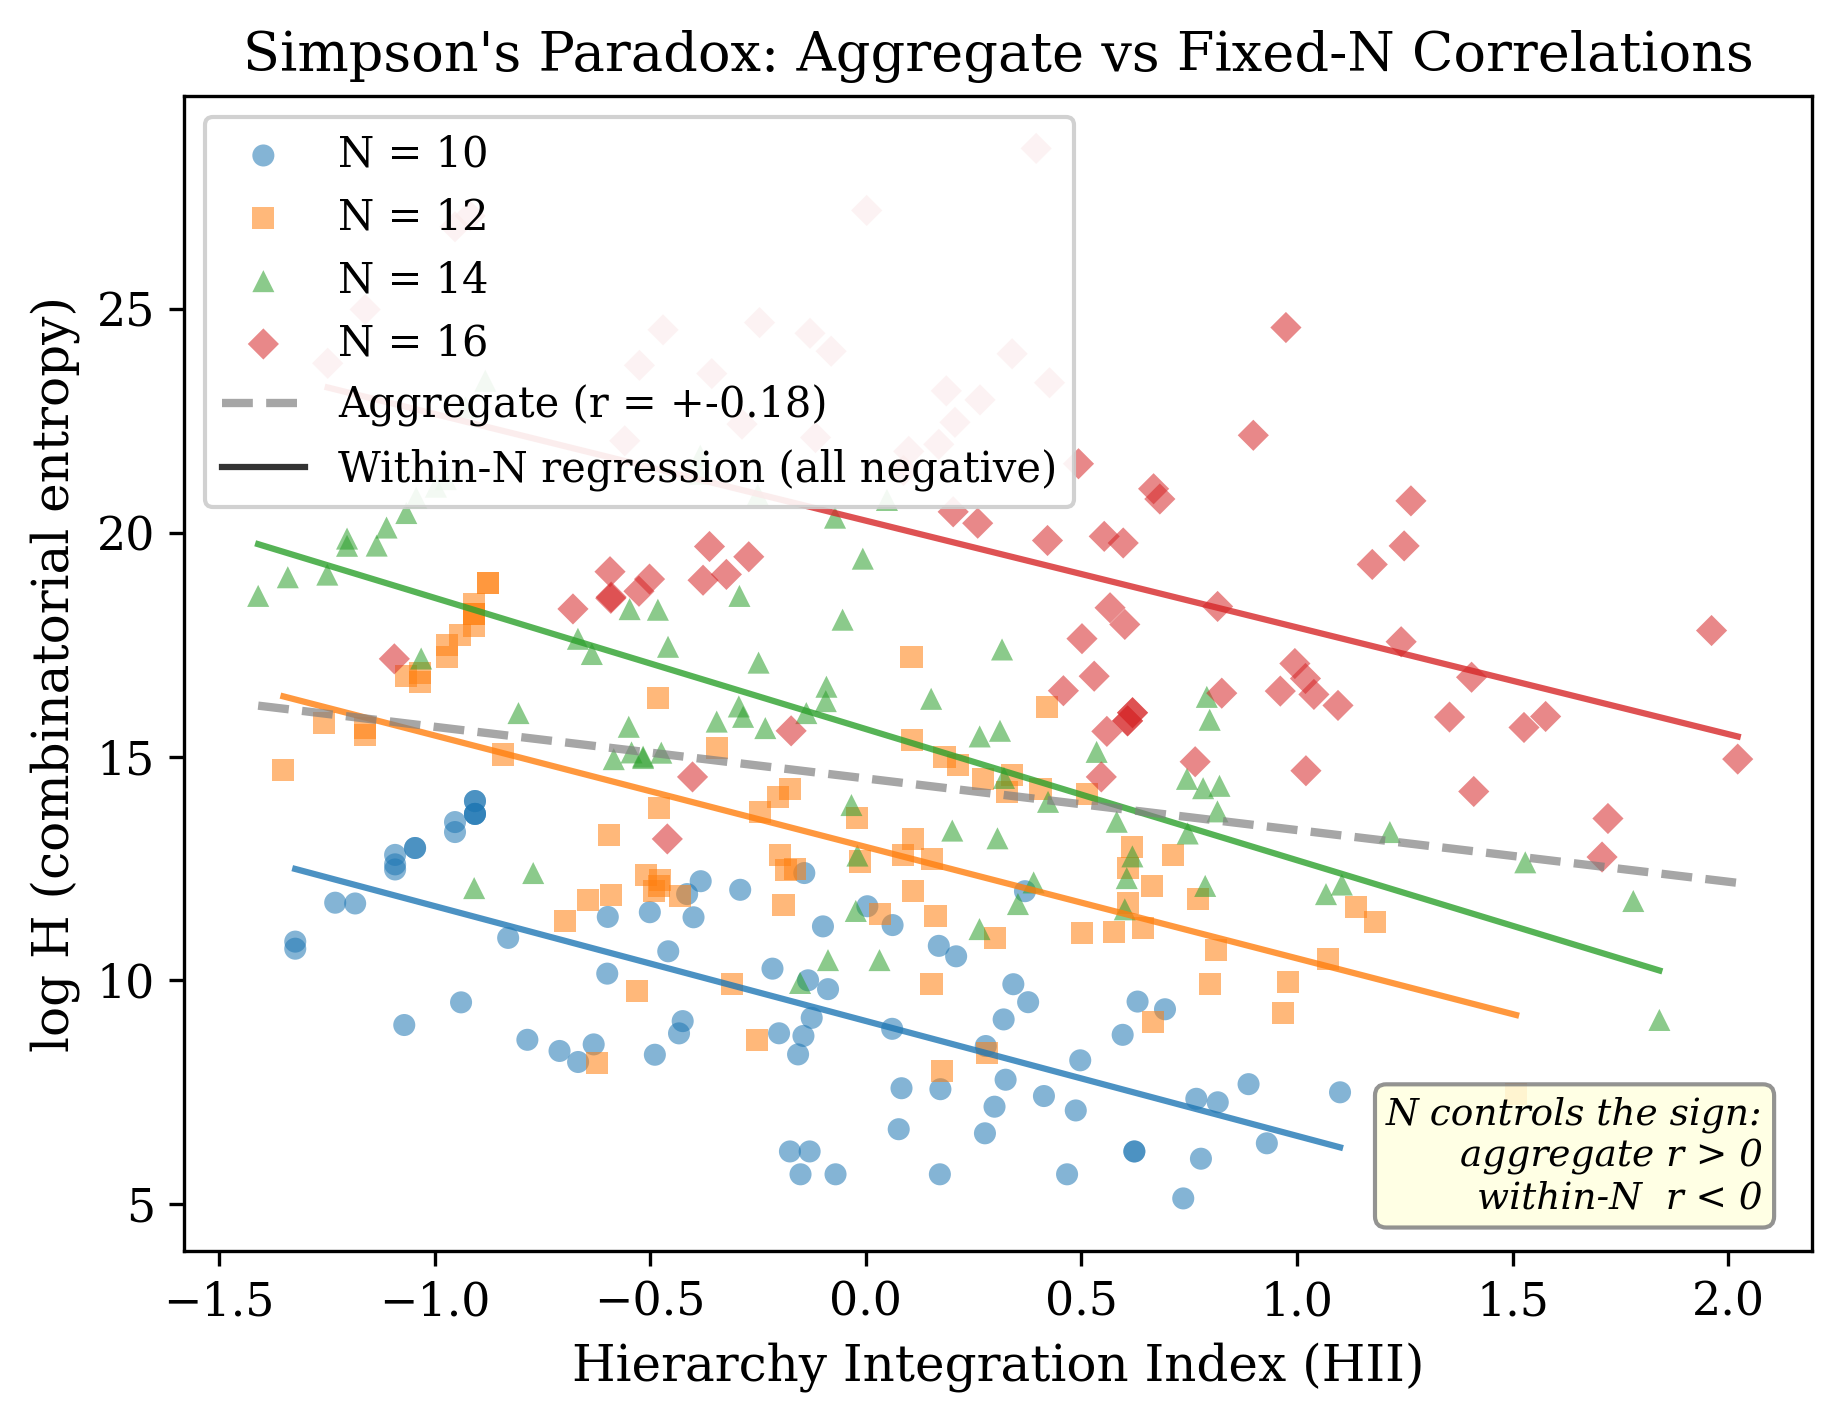
\includegraphics[width=0.9\textwidth]{manuscript_figures/fig1_simpsons_paradox.png}
    \caption{Simpson's Paradox in the HII--$\log H$ relationship. Each colour represents one fixed-$N$ slice ($N = 10, 12, 14, 16$); solid lines show within-$N$ regressions (all negative). The dashed grey line is the aggregate (na\"ive) regression across all $N$ values, which is positive ($r \approx +0.12$). Controlling for $N$ reverses the apparent direction of the correlation.\label{fig:simpson}}
\end{figure}

\subsection{Tier~2: Matched-Pair $\Delta$-Correlation}

Tier~2 uses 46 matched Lor2D--MLR pairs (Table~\ref{tab:tier2_pairs}).

\begin{table}[H]
\caption{Matched-pair dataset composition.\label{tab:tier2_pairs}}
\begin{tabular}{lll}
\toprule
\boldmath$N$ & \textbf{Pairs} & \textbf{Filter} \\
\midrule
30 & 12 & P10--P90 \\
40 & 12 & P10--P90 \\
44 & 6 & P10--P90 \\
48 & 4 & P10--P90 \\
52 & 6 & P5--P95 \\
56 & 6 & P5--P95 \\
\midrule
\textbf{Total} & \textbf{46} & \\
\bottomrule
\end{tabular}
\end{table}

The composite $\text{HII}_\Delta$ achieves $r(\Delta\text{HII}, \Delta\log H) = -0.834$ ($p < 0.001$). All five individual HII components also show the predicted sign direction; \texttt{mean\_layer\_gap} ($r = -0.836$) and \texttt{layer\_count} ($r = -0.816$) nearly match the composite.

\textbf{Sensitivity to filter stringency.}

\begin{table}[H]
\caption{Stability of $r(\Delta\text{HII}, \Delta\log H)$ across three filter windows.\label{tab:sensitivity}}
\begin{tabular}{llllc}
\toprule
\textbf{Filter} & \textbf{Quantile} & \boldmath$N$ \textbf{range} & \textbf{Pairs} & \boldmath$r$ \\
\midrule
Expanded & P10--P90 & 30--48 & 34 & $-0.836$ \\
\textbf{Moderate} & \textbf{P5--P95} & \textbf{30--56} & \textbf{46} & $\mathbf{-0.834}$ \\
Rescue & P0--P100 & 30--56 & 50 & $-0.839$ \\
\bottomrule
\end{tabular}
\end{table}

The correlation coefficient varies by less than 0.005 across the three stringency levels --- a strong robustness check.

\begin{figure}[H]
    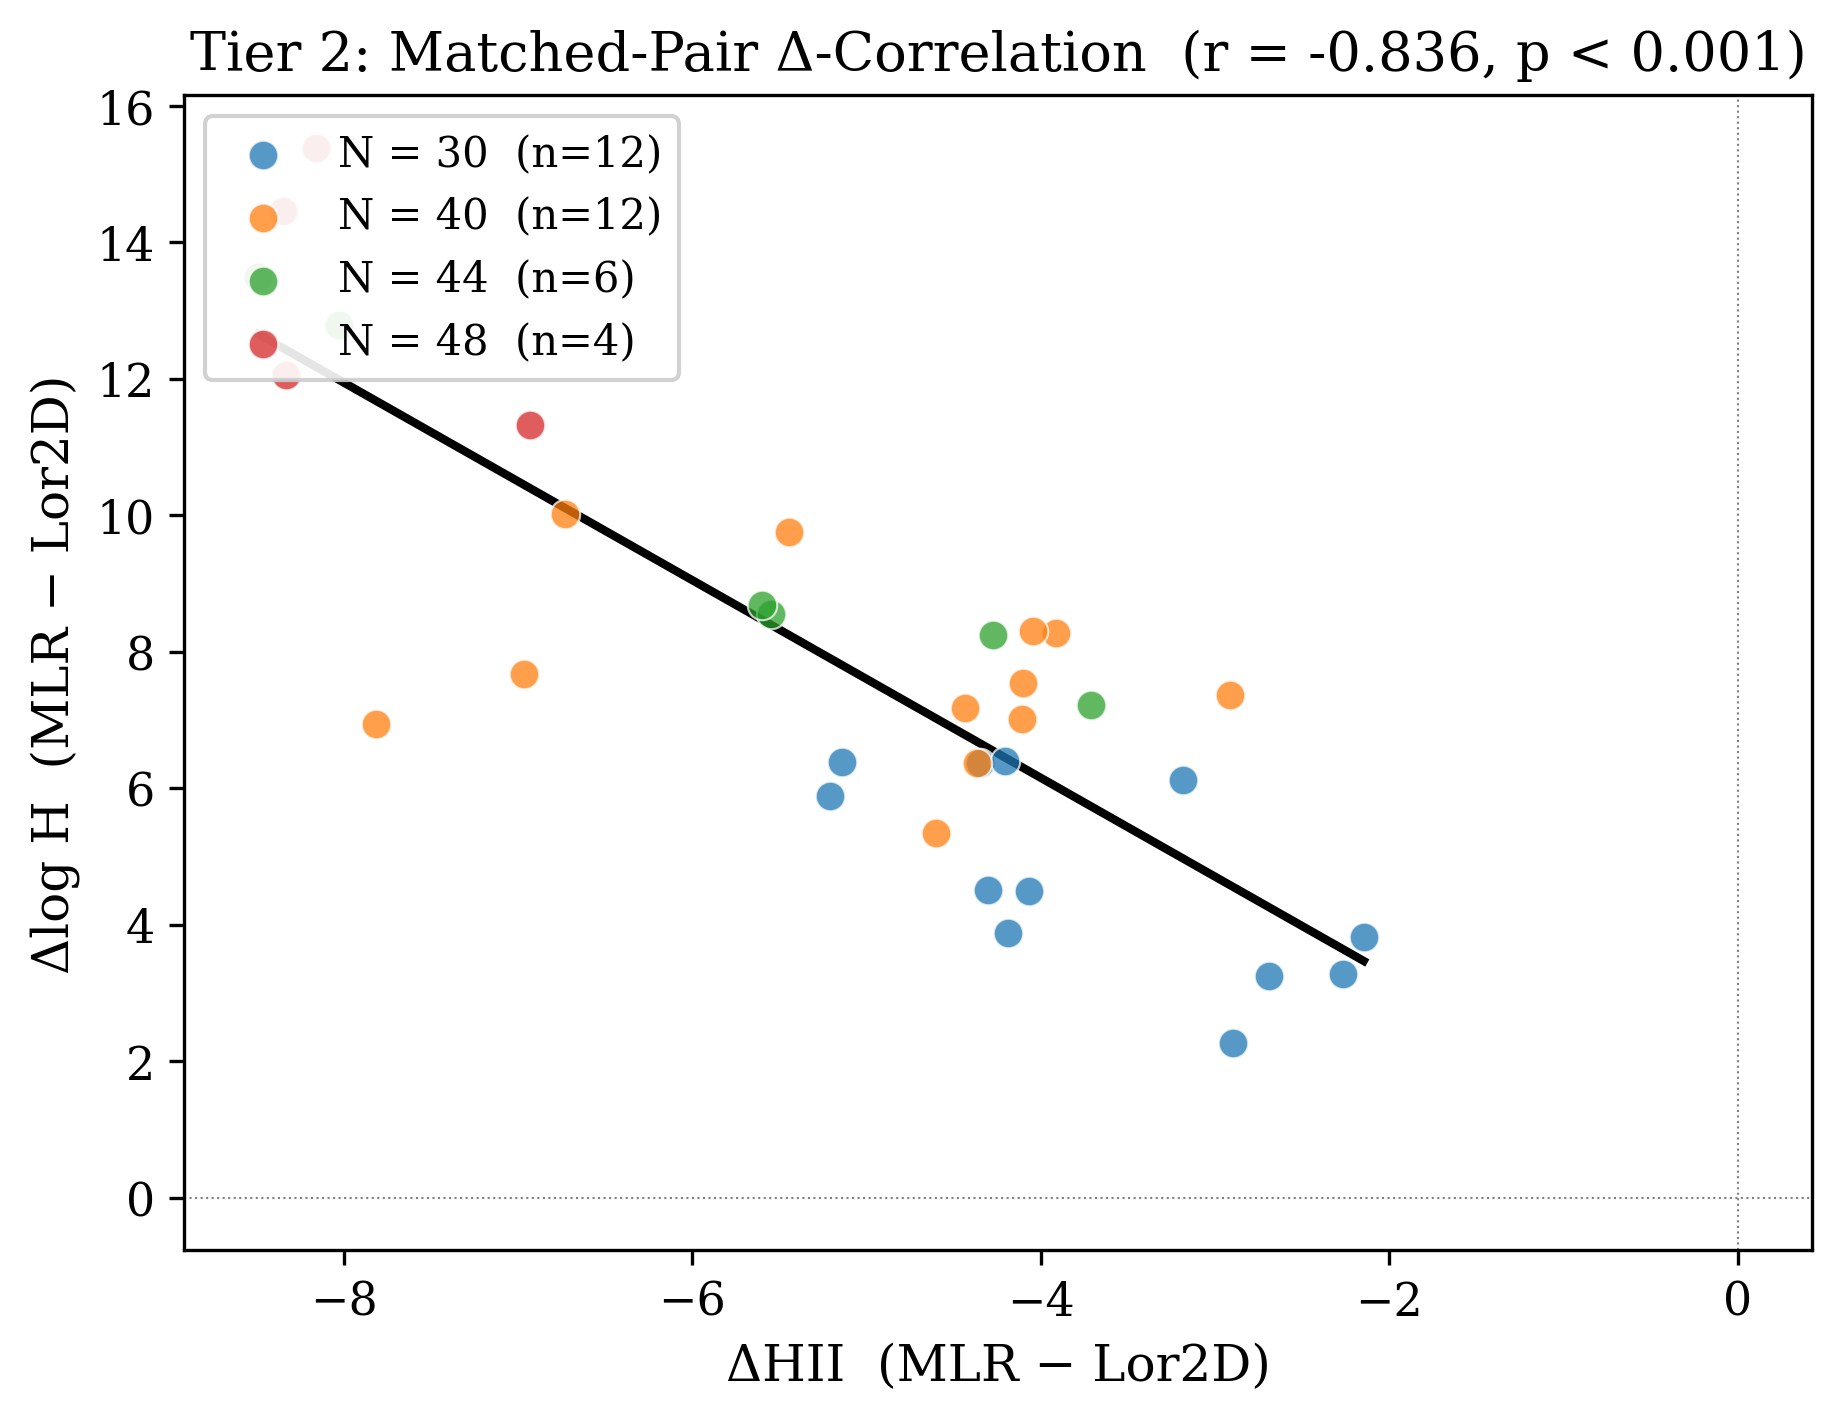
\includegraphics[width=0.9\textwidth]{manuscript_figures/fig2_tier2_delta_correlation.png}
    \caption{Tier~2 matched-pair $\Delta$-correlation. Each point is one Lor2D--MLR pair at the same~$N$; $\Delta\text{HII} = \text{HII}_\text{MLR} - \text{HII}_\text{Lor2D}$ and $\Delta\log H = \log H_\text{MLR} - \log H_\text{Lor2D}$. The black line is the overall linear fit ($r = -0.834$, $p < 0.001$). Colours indicate the poset size~$N$ of each pair.\label{fig:delta}}
\end{figure}

\subsection{Tier~3: Coarse-Graining Stability Linkage}

Tier~3 uses 92 samples (Lor2D + MLR, $N = 30$--$56$). The single strongest predictor of CG stability is \texttt{layer\_count} ($r = -0.874$, $p < 0.001$), surpassing the composite HII ($r = -0.820$). \texttt{mean\_layer\_gap} ($r = -0.847$) and \texttt{long\_edge\_fraction} ($r = -0.803$) also achieve $|r| > 0.8$. This result extends the association chain: deeper hierarchy not only correlates with lower entropy but also with greater identity stability under the current classification protocol.

\subsection{Cross-Tier Summary}

\begin{table}[H]
\caption{Key effect sizes across the three tiers.\label{tab:cross_tier}}
\begin{tabular}{lllccll}
\toprule
\textbf{Tier} & \textbf{Design} & \textbf{Best metric} & \boldmath$r$ & \boldmath$p$ & \boldmath$N$ & \textbf{Samples} \\
\midrule
1 & All-family partial & HII vs $\log H$ ($\mid N$) & $-0.578$ & $<0.001$ & 10--16 & 320 \\
2 & Matched-pair $\Delta$ & $\text{HII}_\Delta$ vs $\Delta\log H$ & $-0.834$ & $<0.001$ & 30--56 & 46 pairs \\
3 & Feature $\to$ $\sigma_\text{CG}$ & layer\_count vs $\sigma_\text{CG}$ & $-0.874$ & $<0.001$ & 30--56 & 92 \\
\bottomrule
\end{tabular}
\end{table}

All three tiers show consistently large negative effect sizes ($|r| > 0.5$), with Tiers~2 and~3 exceeding $|r| = 0.8$. Together, the tiers provide mutually reinforcing correlational support for an association chain:
\begin{equation}
    \text{deeper hierarchy} \;\longrightarrow\; \text{lower entropy} \;\longrightarrow\; \text{greater CG identity stability.}
    \label{eq:chain_full}
\end{equation}

%=================================================================
\section{Simpson's Paradox: Poset Size as the Dominant Sign-Determining Confound}\label{sec:simpson}

\subsection{The Anomaly}

The most counterintuitive result in Tier~1 is the \emph{sign} of the na\"ive partial correlation. Controlling for antichain width, comparable fraction, and geometric dimension gives $r_\text{partial}(\text{HII}, \log H \mid \text{aw, cf, geo\_dim}) = +0.336$ ($p = 0.0005$). This positive sign directly contradicts the prediction. This section shows that it is a Simpson's Paradox driven by~$N$.

\subsection{Stepwise Confound Identification}

\begin{table}[H]
\caption{Stepwise diagnosis of the Simpson's Paradox ($n = 320$).\label{tab:simpson}}
\begin{tabular}{lllll}
\toprule
\textbf{Step} & \textbf{Control variables} & \boldmath$r_\text{partial}$ & \textbf{Sign} & \textbf{Interpretation} \\
\midrule
0 & None (raw Pearson) & $+0.12$ & $+$ & $N$-scaling dominates \\
1 & aw, cf, geo\_dim & $+0.336$ & $+$ & Simpson's Paradox \\
2 & \boldmath$N$ \textbf{only} & $\mathbf{-0.578}$ & $\mathbf{-}$ & Sign flip --- resolved \\
3 & $N$ + family dummies & $-0.250$ & $-$ & Attenuated by within-family noise \\
4 & $N$ + aw + cf + geo\_dim & $-0.434$ & $-$ & Full controls: still negative \\
\bottomrule
\end{tabular}
\end{table}

The diagnostic pattern is clear: $N$ is the dominant sign-determining confound. Adding~$N$ at step~2 produces the largest absolute change in~$r$ ($+0.336 \to -0.578$, a swing of~$0.914$).

\subsection{Why $N$ Is a Confound}

$N$ simultaneously drives both HII and $\log H$, but with different magnitudes:

\begin{enumerate}[nosep]
    \item \textbf{$N \to \log H$}: The number of linear extensions grows combinatorially with $N$. Across all 8 families, $r(N, \log H) > 0.91$. This is a first-order scaling effect.
    \item \textbf{$N \to \text{HII}$}: Larger posets generically admit deeper layer structures, so HII tends to increase with $N$ across families ($r(N, \text{HII}) \approx +0.65$). This is a second-order structural effect.
    \item \textbf{Cross-$N$ contamination}: Without controlling for $N$, the analysis conflates a \emph{scaling effect} (positive: larger $N$ $\Rightarrow$ both HII~$\uparrow$ and $\log H$~$\uparrow$) with a \emph{structural effect} (negative: at fixed $N$, deeper hierarchy $\Rightarrow$ $\log H$~$\downarrow$). Because the scaling effect operates on a larger dynamic range, the aggregate relationship appears positive.
\end{enumerate}

\subsection{An Ecological Correlation}

This is a textbook instance of an \emph{ecological fallacy}: the aggregate-level trend (positive) is the reverse of the within-group trend (negative). The fixed-$N$ Pearson correlations (Table~\ref{tab:fixedN}) confirm this directly: at every $N$ from 10 to 16, the cross-family $r(\text{HII}, \log H)$ is negative.

\subsection{Physical Analogy: Crystallization at Fixed Temperature}

An intuitive analogy: \emph{temperature} plays the role of $N$; crystalline order plays the role of HII; thermodynamic entropy plays the role of $\log H$. At fixed temperature, crystals have lower entropy than liquids because internal structure constrains microstates. Across temperatures, a cold crystal compared to a hot gas gives a misleading positive correlation. Studying the structure--entropy relationship requires \emph{fixing the temperature} (controlling for~$N$).

\subsection{Verification: Family Controls Alone Are Insufficient}

Family dummies alone give $r_\text{partial} = +0.148$ ($p = 0.043$) --- still positive, because within each family, $N$ still acts as a confound. Only explicit $N$ control (or Tier~2's matched-pair design) resolves the paradox.

\subsection{Methodological Implication}

The Simpson's Paradox has a general lesson:

\emph{Raw correlations between structural observables and entropy-like quantities should not be trusted without explicit $N$ control.} The super-linear growth of $\log H$ with $N$ creates confounds that can reverse structural relationships.

%=================================================================
\section{Component Decomposition and Mechanism Refinement}\label{sec:decomposition}

\subsection{Motivation}

The Hierarchy Integration Index is a composite of five z-scored observables:
\begin{equation}
    \text{HII} = \frac{z_\text{lc} + z_\text{mlg} + z_\text{lef} - z_\text{aef} - z_\text{red}}{5},
    \label{eq:hii_expanded}
\end{equation}
where lc = layer\_count, mlg = mean\_layer\_gap, lef = long\_edge\_fraction, aef = adjacent\_edge\_fraction, red = reduction\_edge\_density. Sections~\ref{sec:results} and~\ref{sec:simpson} established strong negative correlation with~$\log H$. This section decomposes the composite into its constituents.

\subsection{Component-Level $\Delta$-Correlations (Tier~2)}

\begin{table}[H]
\caption{Component-level Pearson $r$ with $\Delta_{\log H}$ (46 matched pairs).\label{tab:comp_tier2}}
\begin{tabular}{llll}
\toprule
\textbf{Component} & \boldmath$r(\Delta_\text{comp}, \Delta_{\log H})$ & \boldmath$p_\text{perm}$ & \textbf{Expected sign} \\
\midrule
mean\_layer\_gap & $-0.836$ & $< 0.001$ & $-$ \checkmark \\
\textbf{HII (composite)} & $\mathbf{-0.834}$ & $< 0.001$ & $-$ \checkmark \\
layer\_count & $-0.816$ & $< 0.001$ & $-$ \checkmark \\
long\_edge\_fraction & $-0.643$ & $< 0.001$ & $-$ \checkmark \\
adjacent\_edge\_fraction & $+0.643$ & $< 0.001$ & $+$ \checkmark \\
reduction\_edge\_density & $+0.459$ & $0.001$ & $+$ \checkmark \\
\bottomrule
\end{tabular}
\end{table}

All five components have the predicted sign. The top three --- mean\_layer\_gap, HII, layer\_count --- are nearly indistinguishable ($|r| \in [0.816, 0.836]$).

\subsection{Component-Level CG Stability (Tier~3)}

\begin{table}[H]
\caption{Component-level Pearson $r$ with $\sigma_\text{CG}$ (92 samples, Tier~3).\label{tab:comp_tier3}}
\begin{tabular}{lll}
\toprule
\textbf{Component} & \boldmath$r(\text{comp}, \sigma_\text{CG})$ & \boldmath$p_\text{perm}$ \\
\midrule
\textbf{layer\_count} & $\mathbf{-0.874}$ & $< 0.001$ \\
mean\_layer\_gap & $-0.847$ & $< 0.001$ \\
HII (composite) & $-0.820$ & $< 0.001$ \\
long\_edge\_fraction & $-0.803$ & $< 0.001$ \\
adjacent\_edge\_fraction & $+0.803$ & $< 0.001$ \\
reduction\_edge\_density & $+0.571$ & $< 0.001$ \\
\bottomrule
\end{tabular}
\end{table}

\textbf{layer\_count now leads}, followed by mean\_layer\_gap, with HII in third place. The composite does not exceed its best individual component.

\subsection{Cross-Tier Comparison}

\begin{table}[H]
\caption{Component-level $|r|$ across three analyses.\label{tab:comp_cross}}
\begin{tabular}{lcccc}
\toprule
\textbf{Component} & \textbf{Fixed $N{=}14$} & \textbf{Tier~2 $\Delta$} & \textbf{Tier~3 CG} & \textbf{Rank} \\
\midrule
\textbf{layer\_count} & $0.787$ & $0.816$ & $\mathbf{0.874}$ & \textbf{1st} \\
mean\_layer\_gap & $0.745$ & $\mathbf{0.836}$ & $0.847$ & 2nd \\
long\_edge\_fraction & $0.771$ & $0.643$ & $0.803$ & 3rd \\
adj\_edge\_fraction & $0.771$ & $0.643$ & $0.803$ & 3rd (mirror) \\
red\_edge\_density & $0.693$ & $0.459$ & $0.571$ & 5th \\
HII (composite) & $0.649$ & $0.834$ & $0.820$ & --- \\
\bottomrule
\end{tabular}
\end{table}

Two patterns emerge: (1)~\texttt{layer\_count} is the single strongest predictor in 2 of 3 analyses; (2)~the five-component HII composite never exceeds its best constituent.

\begin{figure}[H]
    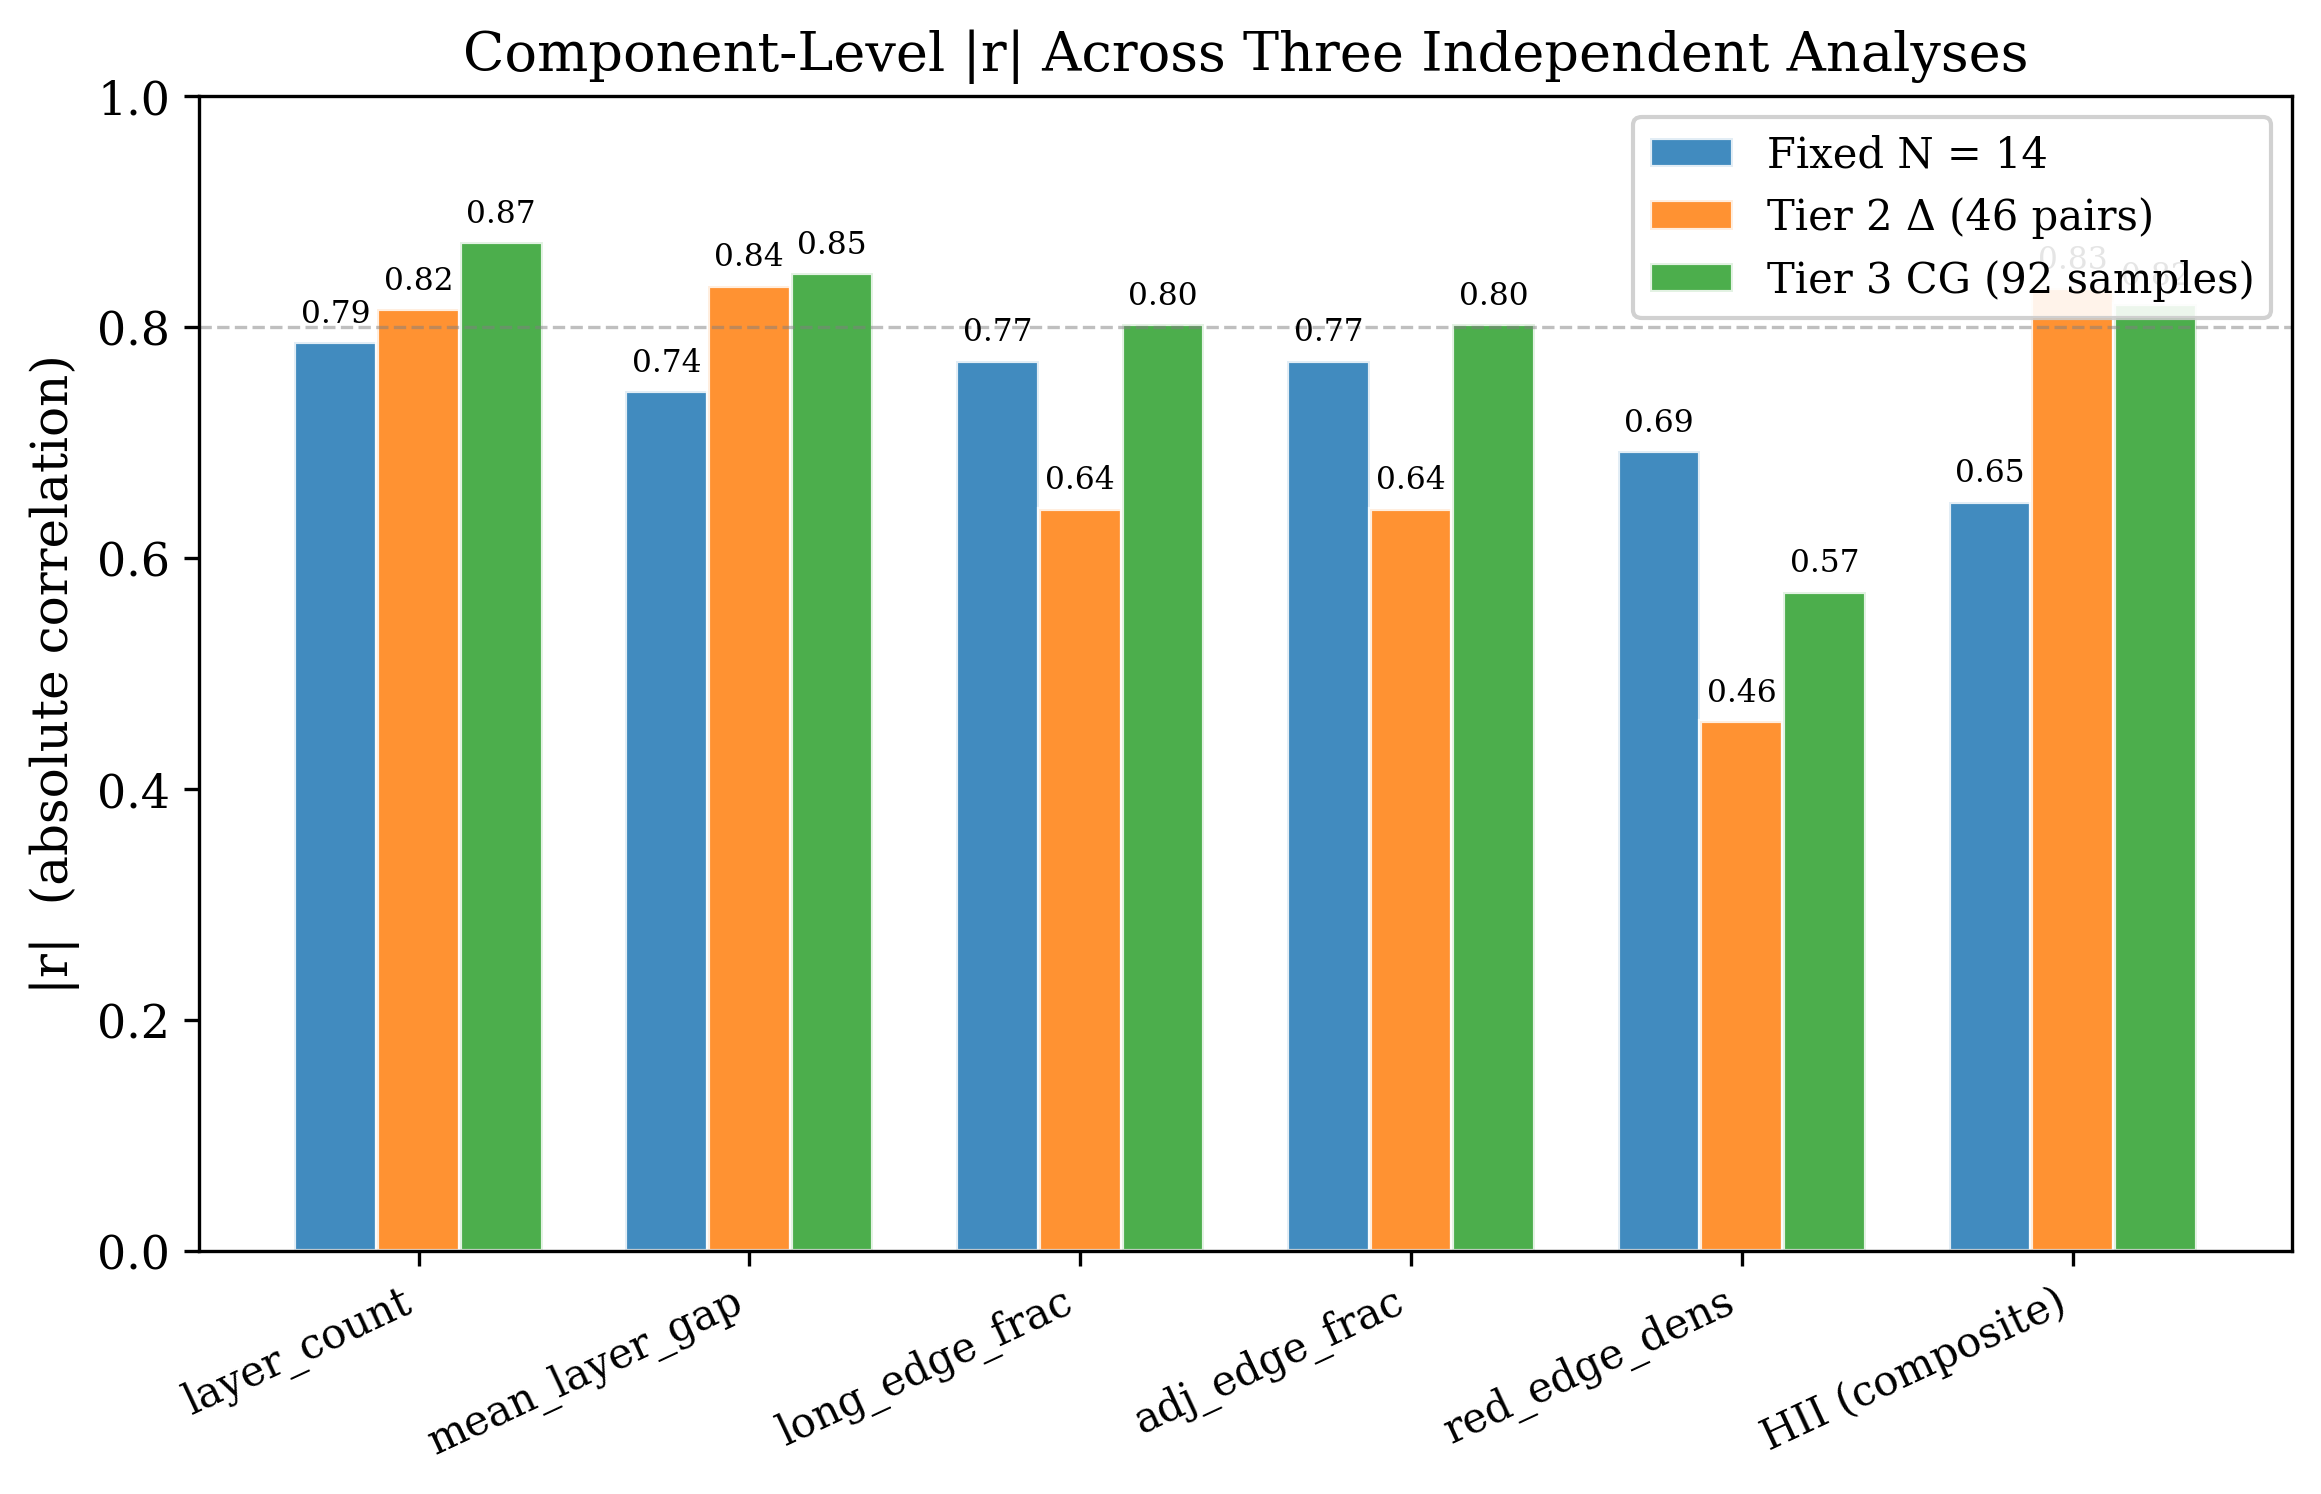
\includegraphics[width=0.95\textwidth]{manuscript_figures/fig3_component_decomposition.png}
    \caption{Component-level absolute correlation $|r|$ across three independent analyses. Blue: fixed $N = 14$ cross-family correlation; orange: Tier~2 matched-pair $\Delta$-method (46 pairs); green: Tier~3 coarse-graining stability (92 samples). The dashed grey line marks $|r| = 0.8$. \texttt{layer\_count} and \texttt{mean\_layer\_gap} consistently dominate; the HII composite never exceeds its best constituent.\label{fig:components}}
\end{figure}

\subsection{Within-Family Behavior at $N = 14$}\label{sec:within_family}

\begin{table}[H]
\caption{Within-family $r(\text{HII}, \log H)$ at $N = 14$ ($n = 10$ per family).\label{tab:within_family}}
\begin{tabular}{lllll}
\toprule
\textbf{Family} & \boldmath$r$ & \textbf{Sign} & \boldmath$p$ & \textbf{HII variability} \\
\midrule
multi\_layer\_random & $-0.861$ & $-$ & $0.001$ & High \\
interval\_order & $-0.746$ & $-$ & $0.013$ & Moderate \\
transitive\_percolation & $-0.678$ & $-$ & $0.031$ & Moderate \\
lorentzian\_like\_3d & $-0.675$ & $-$ & $0.032$ & Moderate \\
lorentzian\_like\_4d & $-0.435$ & $-$ & $0.209$ & Low \\
lorentzian\_like\_2d & $-0.402$ & $-$ & $0.249$ & Moderate \\
absolute\_layered & $+0.294$ & $+$ & $0.410$ & Very low \\
\textbf{KR\_like} & $\mathbf{+0.782}$ & $+$ & $0.008$ & Very low \\
\bottomrule
\end{tabular}
\end{table}

Six of eight families show the predicted negative sign. The two positive outliers --- KR-like and absolute-layered --- have near-constant layer structure by construction. When the primary driver (\texttt{layer\_count}) is clamped, the composite HII loses its predictive content.

\subsection{Physical Interpretation: Layer Depth as the Core Mechanism}

The component decomposition converges on a single structural feature: \textbf{the number of distinct temporal layers} in the poset. Each additional layer imposes a global ordering constraint. For a poset with $k$ layers,
\begin{equation}
    |\mathcal{L}(P)| \leq \prod_{i=1}^{k} |L_i|!\,,
    \label{eq:layer_bound}
\end{equation}
where $L_i$ is the $i$-th antichain-layer. For fixed total $N = \sum_i |L_i|$, increasing $k$ reduces the product combinatorially. The correlation $r(\texttt{layer\_count}, \log H) < 0$ has a transparent combinatorial origin.

\subsection{Implications for Index Refinement}

The data suggest that $\text{HII}_\text{narrow} = (z_\text{layer\_count} + z_\text{mean\_layer\_gap})/2$ would achieve comparable or better predictive power. We do \emph{not} adopt this modification: (1)~the five-component HII was defined \emph{a priori}; (2)~it achieves $|r| > 0.82$ across all controlled analyses; (3)~generalisability should be tested on held-out families.

%=================================================================
\section{Discussion}\label{sec:discussion}

\subsection{Summary of Findings}

This study tested the prediction that deeper hierarchy integration correlates negatively with combinatorial entropy. Three tiers of evidence support this:

\begin{itemize}[nosep]
    \item \textbf{Tier~1}: $r_\text{partial}(\text{HII}, \log H \mid N) = -0.578$; consistent negative sign at each of four $N$ values.
    \item \textbf{Tier~2}: $r(\Delta\text{HII}, \Delta\log H) = -0.834$; stable across three filter stringencies (variation $< 0.005$).
    \item \textbf{Tier~3}: $r(\texttt{layer\_count}, \sigma_\text{CG}) = -0.874$; $r(\text{HII}, \sigma_\text{CG}) = -0.820$.
\end{itemize}

\subsection{What Is Established}

Three claims are supported: (1)~a robust correlational association between hierarchy depth and entropy in cross-family comparisons at fixed~$N$; (2)~a methodological principle that cross-size poset studies must control for~$N$; (3)~correlational support for the association chain (Eq.~\ref{eq:chain_full}).

\subsection{What Is Not Established}

\textbf{Causality.} All three tiers provide correlational evidence only. A causal claim would require an intervention design.

\textbf{Universality.} Results are limited to the eight tested families.

\textbf{Continuum limit.} All analyses operate at finite $N \leq 56$. Whether the correlation persists as $N \to \infty$ is unknown.

\subsection{Relation to Predictions A and B}

Prediction~A~\cite{zhang2026predA} answers \emph{what} is selected. Prediction~B~\cite{zhang2026predB} demonstrates \emph{that} the selection is self-consistent. Prediction~C asks \emph{why}: the answer, within the available evidence, is deeper hierarchy integration.

The three predictions together form a tower (Table~\ref{tab:tower}). The top level is explicitly weaker than the bottom two: A and B make sharp, falsifiable predictions; C establishes a correlational pattern and identifies a mechanism \emph{candidate}.

\subsection{The Near-Wall Boundary}

\begin{table}[H]
\caption{Near-wall survival rates across three filter stringencies.\label{tab:nearwall}}
\begin{tabular}{lccc}
\toprule
\boldmath$N$ & \textbf{P10--P90} & \textbf{P5--P95} & \textbf{P0--P100} \\
\midrule
48 & 4/3468 (0.115\%) & --- & --- \\
52 & 1/60000 (0.002\%) & 6/12601 (0.048\%) & 8/1978 (0.40\%) \\
56 & 0/80000 (0\%) & 6/45121 (0.013\%) & 8/333 (2.4\%) \\
\bottomrule
\end{tabular}
\end{table}

The P10--P90 window is effectively dead at $N \geq 52$. Nevertheless, the Tier~2 correlation is stable across all three levels ($r$ variation $< 0.005$).

\subsection{Limitations}

\begin{enumerate}[nosep]
    \item \textbf{Exact entropy is computationally bounded.} Tier~1 operates at $N \leq 16$; Tiers~2--3 use approximate methods.
    \item \textbf{HII is a bespoke composite.} The component decomposition shows suboptimal weighting. Future work should investigate data-driven weighting on held-out samples.
    \item \textbf{Within-family HII variance is structurally suppressed.} KR-like and absolute-layered have near-constant layer structure by construction.
    \item \textbf{No causal identification strategy.} An intervention design would be needed for causal claims.
    \item \textbf{Two-family matching only.} Tier~2 uses Lor2D--MLR pairs exclusively.
    \item \textbf{Matching quality degrades with $N$.} At $N = 52$--$56$, moderate-filter MLR survivors are structurally less similar to Lor2D.
    \item \textbf{Language boundaries respected throughout.} All findings are stated in correlational terms.
\end{enumerate}

\subsection{Future Directions}

Three directions are natural: (i)~HII refinement on held-out data to test whether a two-component $\text{HII}_\text{narrow}$ matches the full index; (ii)~near-wall generative models to extend Tier~2 beyond $N \approx 60$; (iii)~causal intervention design via controlled layer insertion/removal; (iv)~polynomial-time entropy estimation enabling Tier~1-style analysis at larger scales; (v)~analytic derivation linking layer count to bounds on $|\mathcal{L}(P)|$; (vi)~joint A--B--C modelling to test for mediation effects.

\section{Conclusion}

We have shown that at fixed poset size $N$, hierarchy depth observables --- principally \texttt{layer\_count} and \texttt{mean\_layer\_gap} --- correlate negatively with combinatorial entropy across three independent statistical designs spanning $N = 10$ to $56$. The pre-registered five-component HII composite achieves $|r| > 0.8$ in Tiers~2 and~3, but never exceeds its best constituent; the signal is carried by the depth pair. The correlation is stable across three levels of MLR-filter stringency ($r$ variation $< 0.005$). A Simpson's Paradox in the na\"ive analysis reveals that cross-size comparisons are unreliable without $N$ controls --- a methodological finding of independent value. Hard limitations remain: family-specific reversals (KR-like, absolute-layered), classifier-dependent Tier~3, and weak near-wall power at $N \geq 52$. Within these boundaries, the results provide correlational support for a link between hierarchy depth and entropy suppression in finite causal posets, offering a structural account of \emph{why} certain families achieve lower entropy as observed in Predictions A and B.

%=================================================================
\vspace{6pt}

\authorcontributions{Conceptualization, methodology, software, analysis, writing --- all by the sole author with AI assistance as described in the Acknowledgments.}

\funding{This research received no external funding.}

\dataavailability{All code, configuration files, and output data are available at: \url{https://github.com/unicome37/poset_phase}. Archived version with DOI: \url{https://doi.org/10.5281/zenodo.18980657}.}

\acknowledgments{\textbf{AI Assistance Statement}: This work was conducted in collaboration with large language model assistants (Claude, Anthropic). The AI contributed to experimental design, Python code implementation, data analysis, theoretical interpretation, and manuscript drafting. All scientific decisions, theoretical motivations, and final interpretations were made by the human author, who takes full responsibility for the content.}

\conflictsofinterest{The author declares no conflicts of interest.}

%=================================================================
\begin{adjustwidth}{-\extralength}{0cm}

\reftitle{References}

\begin{thebibliography}{12}

\bibitem{zhang2026predB}
Zhang, G.
Bounded Geometric Phase Transition in Finite Causal Posets with Exact Entropy.
Preprint (2026). \url{https://doi.org/10.5281/zenodo.19048146}.
Code and data: \url{https://doi.org/10.5281/zenodo.18980657}.

\bibitem{zhang2026predA}
Zhang, G.
Dimensional Selection Without Dimensional Priors: 4D Lorentzian Dominance in Finite Causal Poset Ensembles Under Consistency-Based Actions.
Preprint (2026). \url{https://doi.org/10.5281/zenodo.19068927}.
Code and data: \url{https://doi.org/10.5281/zenodo.18980657}.

\bibitem{bombelli1987}
Bombelli, L.; Lee, J.; Meyer, D.; Sorkin, R.D.
Space-Time as a Causal Set.
\textit{Phys.\ Rev.\ Lett.} \textbf{1987}, \textit{59}, 521.

\bibitem{sorkin2005}
Sorkin, R.D.
Causal Sets: Discrete Gravity.
In \textit{Lectures on Quantum Gravity}; Gomberoff, A., Marolf, D., Eds.; Springer: Berlin, Germany, 2005.
arXiv:gr-qc/0309009.

\bibitem{surya2019}
Surya, S.
The Causal Set Approach to Quantum Gravity.
\textit{Living Rev.\ Relativ.} \textbf{2019}, \textit{22}, 5.
https://doi.org/10.1007/s41114-019-0023-1.

\bibitem{surya2012}
Surya, S.
Evidence for the Continuum in 2D Causal Set Quantum Gravity.
\textit{Class.\ Quantum Grav.} \textbf{2012}, \textit{29}, 132001.
https://doi.org/10.1088/0264-9381/29/13/132001.

\bibitem{benincasa2010}
Benincasa, D.M.T.; Dowker, F.
The Scalar Curvature of a Causal Set.
\textit{Phys.\ Rev.\ Lett.} \textbf{2010}, \textit{104}, 181301.
https://doi.org/10.1103/PhysRevLett.104.181301.

\bibitem{kleitman1975}
Kleitman, D.J.; Rothschild, B.L.
Asymptotic Enumeration of Partial Orders on a Finite Set.
\textit{Trans.\ Amer.\ Math.\ Soc.} \textbf{1975}, \textit{205}, 205--220.

\bibitem{brightwell1991}
Brightwell, G.; Winkler, P.
Counting Linear Extensions.
\textit{Order} \textbf{1991}, \textit{8}, 225--242.

\bibitem{henson2006}
Henson, J.
The Causal Set Approach to Quantum Gravity.
In \textit{Approaches to Quantum Gravity}; Oriti, D., Ed.; Cambridge University Press: Cambridge, UK, 2009.
arXiv:gr-qc/0601121.

\bibitem{dowker2005}
Dowker, F.
Causal Sets and the Deep Structure of Spacetime.
In \textit{100 Years of Relativity}; Ashtekar, A., Ed.; World Scientific: Singapore, 2005.
arXiv:gr-qc/0508109.

\bibitem{pratt1981}
Pratt, J.W.; Gibbons, J.D.
\textit{Concepts of Nonparametric Theory}; Springer: New York, NY, USA, 1981.

\end{thebibliography}

\end{adjustwidth}

\end{document}
